\subsection[Restrições de Arquitetura]{Restrições de Arquitetura}

Esta seção fornece uma visão geral sobre as restrições propostas por Fielding para a implementação em arquiteturas web, além de ser examinado o impacto de cada restrição nesses sistemas distribuídos. \\

\textbf{Cliente-Servidor} \\

Nesta primeira restrição, não existe conexão entre cliente e servidor, mas sim a espera do servidor por pedidos de clientes através de chamada e resposta. O cliente (consumidor do serviço) não se preocupa com tarefas de comunicação de banco de dados, gerenciamento de cache, entre outros. Assim como o servidor (prestador de serviços) não está preocupado com as tarefas do cliente como interface ou experiência do usuário por exemplo. Permitindo a evolução independente dos dois ambientes, \textit{desde que sua interface de comunicação não seja alterada}. \cite{Fielding2000} \\

\textbf{Sem Estado} \\

Esta restrição ajuda na viabilidade, confiabilidade e escalabilidade de sistemas distribuídos, pois garantem que chamadas à API não estejam vinculadas a um determinado servidor. Como HTTP é um protocolo sem conexão, cada requisição deve conter todas as informações necessárias para que um servidor entenda o que um cliente está executando. Para Wildermuth, no entanto, dependendo da diversidade no número de clientes, ao manter um servidor sem estado, perder-se o controle no tamanho da estrutura de resposta necessária para atender a demanda de todos os clientes. \cite{Wildermuth2015} \\

\textbf{Interface Uniforme} \\

Em essência, Fielding propõe que aplicações façam o uso de verbos HTTP (POST, GET, PUT, DELETE) e identificadores uniforme de recursos (URI) para mapear operações em ambientes distribuidos e minimizar o acoplamento entre cliente-servidor. Essas regras de acesso são: \cite{Fielding2000}

\begin{itemize}[noitemsep]
\item Identificação de Recursos: Cada recurso deve ser disponibilizado através de uma URI específica e coesa. (Exemplo: GET /customers/1)
\item Manipulação de Recursos através de Representações: Um recurso pode ser representado em diferentes formatos para diferentes clientes. (Exemplo: HTML, XML, JSON)
\item Resposta Auto-explicativa: Metadados devem ser adicionados na requisição e resposta de um recurso para descrever seu estado atual ou desejado. (Exemplo: código de resposta HTTP, Host, Content-Type)
\item HATEOAS\footnote{
  Hypermedia as the Engine of Application State.
} - Caso um recurso possua relacionamentos, ao ser representado, estes devem estar especificados em forma de hiperlinks para facilitar a navegação de dados por clientes.
\end{itemize}

\textbf{Separação em Camadas} \\

Um dos princípios desta restrição está em evitar que clientes façam diretamente requisição para o servidor sem antes passar por um intermediário, como por exemplo um load balancer\footnote{
  Técnica para distribuir a carga de trabalho uniformemente entre dois ou mais computadores
}. Assegurando que clientes apenas se preocupem com a comunicação, deixando para que intermediários lidem com a distribuição de requisições. \cite{Fielding2000}

\begin{figure}[H]
  \centering  	   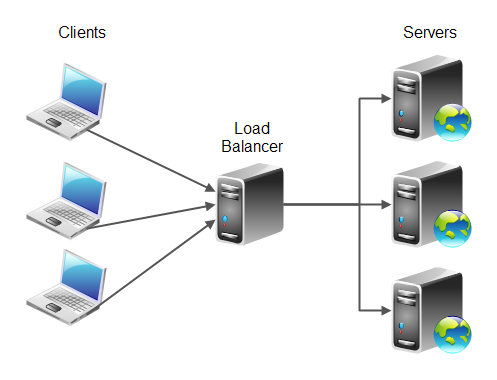
\includegraphics[width=0.6\textwidth,height=\textheight,keepaspectratio]{figuras/load-balancer.png}
  \caption{Exemplo de Load Balancer}
\end{figure}

\textbf{Código sob Demanda} \\

Apesar de ser a única restrição opcional do estilo, ela permite que servidores disponibilizem código em forma de script para que seja executado no cliente. Dessa forma, extendendo a lógica de serviço do servidor para seus clientes. \cite{Fielding2000} \\

\textbf{Cache} \\

Para aumentar desempenho de um serviço. Quando um recurso é acessado por mais de um cliente, se não houve mudança é recomendado que a resposta seja armazenada em cache, evitando o processamento desnecessário. Isso significa que servidores, quando possível, devem implementar regras de cache para beneficio de ambos os ambientes. \cite{Fielding2000}
